\chapter{GPU-based Parallel Collision Checking} 
\label{chp:GCollide}


\section{Introduction}
It is known that a significant fraction (i.e., $90\%$ or more) of randomized sampling algorithms is
spent in collision checking. This includes checking whether a given configuration is in free-space or not,
as well as connecting two free-space configurations using a local planning algorithm. In Chapter~\ref{chp:GPlanner}, we exploit the computational power and massive parallelism of commodity GPUs (graphics processing units) for almost real-time
computation. To enable this, we need to design appropriate parallel collision algorithms that can map well to GPUs.

\subsection{Main Results}
We present a novel, parallel algorithm for performing collision queries for sample-based
motion planning. Our approach exploits parallelism at two levels: it checks multiple configurations simultaneously (to determine whether they are in free space or not) and performs parallel hierarchy traversal for each collision query.
Similar techniques are also used for local planning queries. We use clustering techniques to appropriately
allocate the collision queries to different cores. Furthermore, we introduce the notion of \emph{collision-packet traversal},
which ensures that all the configurations allocated to a specific core result in similar hierarchical traversal
patterns. The resulting approach also exploits fine-grained parallelism which uses bounding volume overlap tests
to balance the workload.

The resulting algorithms have been implemented on commodity NVIDIA GPUs. In practice, we are able to process about
$500,000$ collision queries per second on a \$400 NVIDIA GeForce 480 desktop GPU, which is almost 10 times faster than prior GPU-based collision checking algorithms. We also use our collision checking algorithm for GPU-based motion planners of high-DOF
rigid and articulated robots.
The resulting planner can compute collision-free paths in less than $100$ milliseconds for various benchmarks and
appears to be $50\text{-}100$ times faster than CPU-based PRM planners.

\subsection{Organization}
The rest of this chapter is organized as follows. We survey related work on collision detection
algorithms in Section~\ref{sec:5:related}. Section~\ref{sec:5:overview} gives an overview of our approach, and we present parallel algorithms
for collision queries in Section~\ref{sec:5:algorithm}. We evaluate the performance of our algorithm on different benchmarks in Section~\ref{sec:5:result}.

\section{Related Work}
\label{sec:5:related}
In this section, we give a brief overview of prior work in parallel algorithms for collision
detection.

\subsection{Parallel Collision Queries}
Some of the widely-used algorithms for collision checking are based on \emph{bounding volume hierarchies} (BVH),
such as $k$-DOP trees, OBB trees, AABB trees, and so forth~\cite{LM03}. Recent developments include parallel hierarchical computations on multi-core CPUs~\cite{Kim08,TMT10-GMOD} and GPUs~\cite{Lauterbach10}. CPU-based approaches tend to rely on fine-grained communication
between processors, which is not suited for current GPU-like architectures. On the other hand, GPU-based
algorithms~\cite{Lauterbach10} use work queues
to parallelize the computation on multiple cores. All of these approaches are primarily designed to parallelize a
single collision query.

However, the capability to efficiently perform high numbers of collision queries is essential in motion planning algorithms; for example, multiple collision queries are used in milestone computation and local planning. Some existing algorithms
perform parallel queries in a simple manner: each thread handles a single collision query independently~\cite{Amato99,akinc+2003:prt-p}. Since current multi-core CPUs have the capability to perform \emph{multiple-instruction multiple-data} (MIMD) computations, these simple strategies can work well on CPUs.
On the other hand, current GPUs offer high data parallelism and the ability to execute a high number of threads
in parallel to overcome high memory latency. As a result, we need new parallel collision detection algorithms
to fully exploit the capabilities of GPUs.

\section{Overview}
\label{sec:5:overview}
In this section, we address
some issues in designing efficient parallel algorithms to perform collision queries.

\subsection{Notation and Terminology}
We define some terms and symbols used in the rest of this chapter.
\begin{description}
\item[chunk] The minimum number of threads that GPUs manage, schedule and execute in parallel, which is also called \emph{warp} in GPU computing literature. The size of each chunk (\emph{chunk-size} or \emph{warp-size}) is 32 on current NVIDIA GPUs (e.g., GTX 280 and 480).
\item[block] The logical collection of GPU threads that can be executed on the same GPU core. These threads synchronize by using barriers
and communicate via a small high-speed low-latency \emph{shared memory}.
\item[BVH$_a$] The \emph{bounding volume hierarchy} (BVH) tree for model $a$. It is a binary tree with $L$ levels, with nodes ordered in breadth-first order starting from the root node. The $i$-th BVH node is denoted as BVH$_a[i]$ and its children nodes are
BVH$_a[2i]$ and BVH$_a[2i+1]$ with $1\leq i \leq 2^{L-1}-1$. The nodes at the $l$-th level of a BVH tree are represented as
BVH$_a[k], 2^l \leq k \leq 2^{l+1} - 1$ with $0
\leq l < L$. The inner nodes are also called \emph{bounding volumes} (BV), and the leaf nodes also have a link to the primitive
triangles that are used to represent the model.
\item[BVTT$_{a,b}$] The \emph{bounding volume test tree} (BVTT) represents recursive collision query traversal between two
objects $a$ and $b$. It is a 4-ary tree, whose nodes are ordered in breadth-first order starting from the root node. The $i$-th BVTT node is denoted as BVTT$_
{a,b}[i]\equiv ($BVH$_a[m]$, BVH$_b[n])$ or simply $(m, n)$, which checks the BV or primitive overlap between nodes BVH$_a[m]$ and BVH$_b[n]$. Here $m = \lfloor i - \frac{4^M + 2}{3} \rfloor + 2^M$, $n = \{i - \frac{4^M + 2}{3}\} + 2^M$ and $M = \lfloor \log_4(3i -
2) \rfloor$, where $\{x\} = x - \lfloor x \rfloor$. BVTT node $(m, n)$'s children are $(2m, 2n)$, $(2m, 2n+1)$, $(2m+1,2n)$, and $(2m+1,2n+1)$.
\item[$\mathbf{q}$] A configuration of the robot, which is randomly sampled within the
configuration space ($\mathcal{C}$-Space).  $\mathbf{q}$ is associated with the transformation $\mathbf{T}_{\mathbf{q}}$.
The BVH of a model $a$ after applying such a transformation is given as BVH$_a(\mathbf{q})$.
\end{description}

The relationship between BVH trees and BVTT is also shown in Figure~\ref{fig:5:BVTT}. Notice that given the BVHs
of two geometric models, the BVTT is completely determined using those BVHs and is independent of the actual configuration of
each model. The model configurations only affect the actual traversal path of the BVTT.

\begin{figure}[!h]
  \centering
  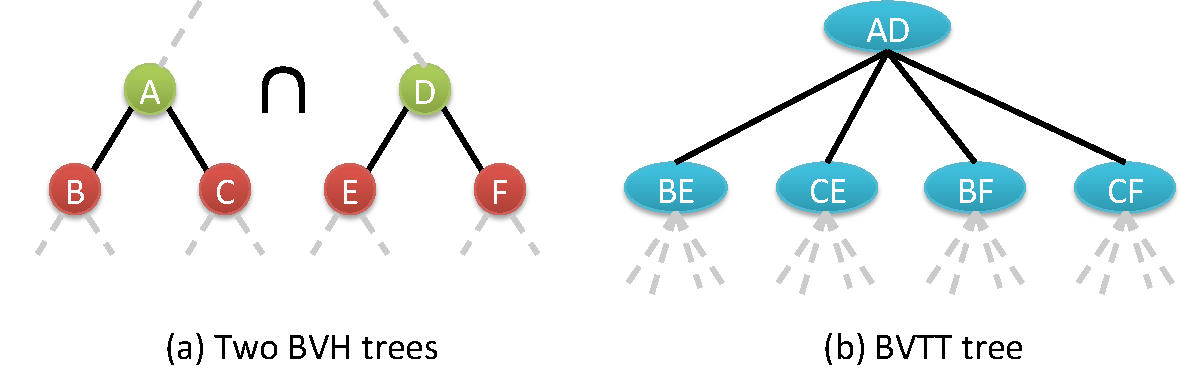
\includegraphics[width=\linewidth]{figs/5/BVTT.pdf}
  \caption[Illustrations of BVH and BVTT]{BVH and BVTT: (a) shows two BVH trees and (b) shows the BVTT tree for the collision checking between the two BVH trees.}
  \label{fig:5:BVTT}
\end{figure}

\subsection{Collision Queries: Hierarchical Traversal}
Collision queries between the geometric models are usually accelerated with hierarchical techniques based on BVHs,
which correspond to traversing the BVTT~\cite{LGLM00}. The simplest parallel algorithms
used to perform multiple collision queries involve each thread traversing the BVTT for a single configuration and checking whether the given configuration is
in free space or not. This simple parallel algorithm is shown in Algorithm~\ref{algo:5:naive}. This
strategy is easy to implement and has been used in previous parallel planning algorithms based on multi-core or multiple CPUs.
However, it may not result in high parallel efficiency on current GPUs due to the following reasons.
\begin{algorithm}[htb]
    \caption{Simple parallel collision checking; such approaches are widely used on multi-core CPUs}
    \label{algo:5:naive}
    \begin{algorithmic}[1]
    \STATE Input: $N$ random configurations $\{\mathbf{q}_i\}_{i=1}^N$, BVH$_a$ for the robot and BVH$_b$ for the obstacles
    \STATE Output: return whether one configuration is in free space or not
    \STATE $t_{id} \leftarrow $ thread id of the current thread
    \STATE $\mathbf{q} \leftarrow \mathbf{q}_{t_{id}}$
    \STATE $\lhd$ traversal stack $S$[] is initialized with root nodes
    \STATE \textbf{shared}/\textbf{global} $S$[] $\equiv$ local traversal stack
    \STATE $S$[] $\leftarrow $BVTT$[1] \equiv ($BVH$_a(\mathbf{q})[1],$BVH$_b[1])$
    \STATE $\lhd$ traverse BVTT for BVH$_a(\mathbf{q})$ and BVH$_b$
    \LOOP
    \STATE $(x,y) \leftarrow \pop(S)$.
    \IF{$\overlap($BVH$_a(\mathbf{q})[x],$BVH$_b[y])$}
        \IF{!$\isLeaf(x)$ \&\& !$\isLeaf(y)$}
            \STATE $S$[] $\leftarrow (2x,2y),(2x,2y+1),(2x+1,2y),(2x+1,2y+1)$
        \ENDIF
        \IF{$\isLeaf(x)$ \&\& !$\isLeaf(y)$}
            \STATE $S$[] $\leftarrow (2x,2y),(2x,2y+1)$
        \ENDIF
        \IF{!$\isLeaf(x)$ \&\& $\isLeaf(y)$}
            \STATE $S$[] $\leftarrow (2x,2y),(2x+1,2y)$
        \ENDIF
        \IF{$\isLeaf(x)$ \&\& $\isLeaf(y)$\&\& \\ $\exactIntersect($BVH$_a(\mathbf{q})[x],$BVH$_b[y])$}
            \STATE \textbf{return} $collision$
        \ENDIF
    \ENDIF
    \ENDLOOP
    \STATE \textbf{return} $collision\text{-}free$
    \end{algorithmic}
\end{algorithm}
First, each thread needs a local traversal stack for the BVTT, which is difficult for GPUs to store. The stack size should be at least $3 (\log_4(N_a) + \log_4(N_b)))$ to avoid stack overflow, where $N_a$ and $N_b$ are the number of primitive triangles in BVH$_a$ and
BVH$_b$, respectively.
The stack can be implemented using either global memory or shared memory. Global memory access on GPUs tends to be slow,
which affects BVTT traversal. Shared memory access is much faster but it may be too small to hold
the large stack for complex geometric models composed of thousands of polygons, and increasing the shared memory usage will limit the extent of parallelism.
Second, different threads may traverse the BVTT tree with incoherent patterns: there are many branching
decisions performed during the traversal (e.g., \textbf{loop}, \textbf{if}, \textbf{return} in the pseudo-code), and the traversal
flow of the hierarchy in different threads diverges quickly. Finally, different threads can have varying workloads, some may be
busy with the traversal while other threads may have finished the traversal early and are idle because
there is no BV overlap or a primitive collision has already been detected. These factors can negatively affect the
performance of the parallel algorithm.

The problems of low parallel efficiency in Algorithm~\ref{algo:5:naive} become more severe in complex and/or
articulated models. For such models, there are longer traversal paths in the hierarchy and the differences between
the lengths of these paths can be large for different configurations of a robot. As a result, differences in the
workloads of different threads can be high, which negatively affects parallelism. For articulated models, each thread checks the collision status
of all the links and stops when a collision is detected for any link. Thus, more branching decisions
are performed within each thread, which can lead to more incoherent traversal.
Similar issues also arise during local planning, when each thread determines whether two milestones
can be joined by a collision-free path by checking for collisions along the trajectory connecting them.



\section{Parallel Collision Detection on GPUs}
\label{sec:5:algorithm}


In this section, we present two novel algorithms for efficient parallel collision checking on GPUs between rigid and articulated models. Our methods check whether a configuration lies in the free space or to perform local planning computations. The first algorithm uses clustering techniques and fine-grained packet-traversal to improve the
coherence of BVTT traversal for different threads. The second algorithm uses queue-based techniques and lightweight workload
balancing to achieve higher parallel performance on the GPUs. In practice, the first method can provide 30\%-50\% speed up.
Moreover, it preserves the per-thread per-query structure of the naive parallel strategy. Therefore, it is easy to implement
and is suitable for cases where we need to perform additional computations (e.g., retraction for handling narrow passages~\cite{Zhang08-ICRA}). The second method can provide 5 to 10-fold speed up, but is relatively more complex to implement.


\subsection{Parallel Collision-Packet Traversal}
\label{sec:5:algorithm:packet}
Our goal is to ensure that all the threads in a block that are performing BVTT-based collision checking have similar workloads and coherent
branching patterns. Our approach is motivated by recent developments related to interactive ray-tracing on GPUs for visual
rendering. Each collision query traverses the BVTT and performs node-node or primitive-primitive intersection tests. In comparison,
ray-tracing algorithms traverse the BVH tree and perform ray-node or ray-primitive intersections. Thus, parallel ray-tracing
algorithms on GPUs also need to avoid incoherent branches and varying workloads to achieve higher performance.

In real-time ray tracing, one approach handling the varying workloads and incoherent branches is the
use of ray-packets~\cite{Gunther07,Aila2009}. In ray-tracing terminology, packet traversal implies that a group of
rays follow
exactly the same traversal path in the hierarchy. This is achieved by sharing the traversal stack (similar to the BVTT traversal stack in Algorithm~\ref{algo:5:naive}) among the rays in the same warp-sized packet (i.e., threads that fit in one chunk on the GPU), instead of each thread using an independent stack for a single ray.
This implies that some additional nodes in the hierarchy may be visited during ray intersection tests, even though there are no intersections between the rays and those nodes. But the resulting traversal is coherent for different rays, because each node is fetched only once per packet. In order to reduce the number of computations (i.e., unnecessary node intersection tests), all the rays in one packet should be similar to one another, i.e., have similar traversal paths with few differing branches. For ray tracing, the packet construction is simple: as shown in Figure~\ref{fig:5:raypacket}, rays passing through the same pixel on the image space make a natural packet. We extend this idea to parallel collision checking and refer to our algorithm as the \emph{multiple configuration-packet} method.

\begin{figure}[!htb]
  \centering
  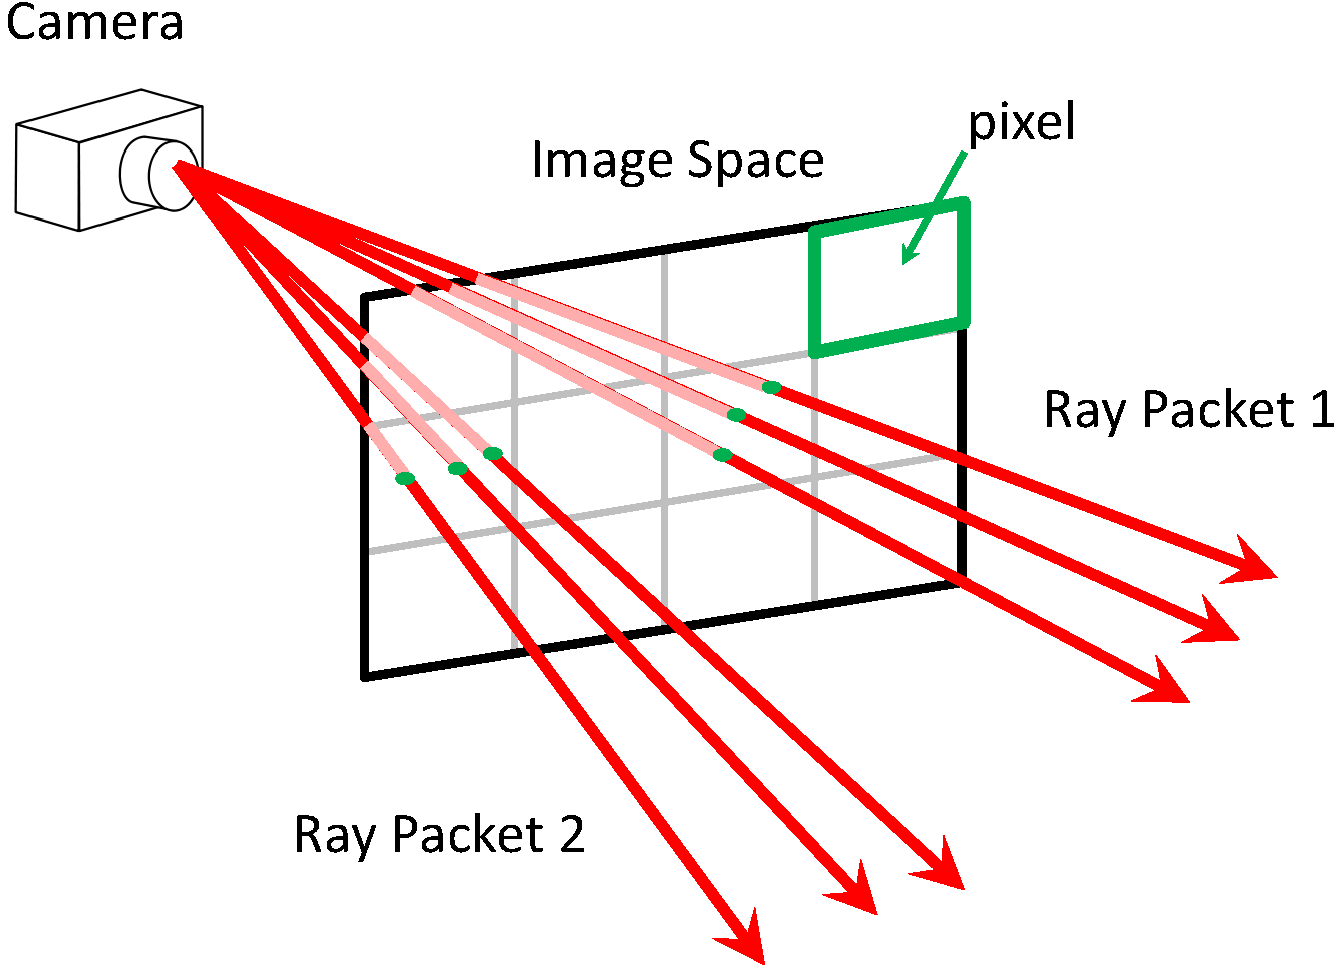
\includegraphics[width=\linewidth]{figs/5/raypacket.pdf}
  \caption[Ray packets for faster GPU-based ray tracing]{Ray packets for faster ray tracing. Nearby rays constitute a ray packet and this spatial coherence is
  exploited for fast intersection tests.}
  \label{fig:5:raypacket}
\end{figure}

The first challenge is to cluster similar collision queries into groups, because unlike
ray tracing, there are no natural packet construction rules for collision queries. In some cases, the sampling scheme (e.g., the adaptive sampling for lazy PRM) can provide natural group partitions. However, in most cases
we need suitable algorithms to compute these clusters. Clustering algorithms are natural choices for such a task; they aim
to partition a set $\mathcal{X}$ of $N$ data items $\{\mathbf{x}_i\}_{i=1}^N$ into $K$ groups $\{C_k\}_{k=1}^K$ such that the data items belonging to the same group are more ``similar" than the data items in different groups. The clustering algorithm
used to group the configurations needs to satisfy some additional constraints: $|C_k| = \text{chunk-size}, 1\leq k \leq K$, where $K = \lceil \frac{N}{\text{chunk-size}} \rceil$. That is, each cluster should fit in one chunk on GPUs, except for the last cluster. Using the formulation of $k$-means, the clustering problem can be formally described as:

\noindent Compute $K = \lceil \frac{N}{\text{chunk-size}} \rceil$ items $\{\mathbf{c}_k\}_{k=1}^K$ that minimizes
\begin{equation}
\label{eq:5:cluster}
\sum_{i=1}^N\sum_{k=1}^K \mathbf{1}_{\mathbf{x}_i \in C_k} \|\mathbf{x}_i - \mathbf{c}_k\|,
\end{equation}
with constraints $|C_k| = \text{chunk-size}, 1\leq k \leq K$. To our knowledge, there are no existing clustering algorithms designed
for this specific problem. One possible solution is to use \emph{clustering with balancing constraints}~\cite{Banerjee:2006},
which has the additional constraints $|C_k| \geq m, 1\leq k \leq K$, where $m \leq \frac{N}{K}$.

\begin{figure}[!htb]
\centering
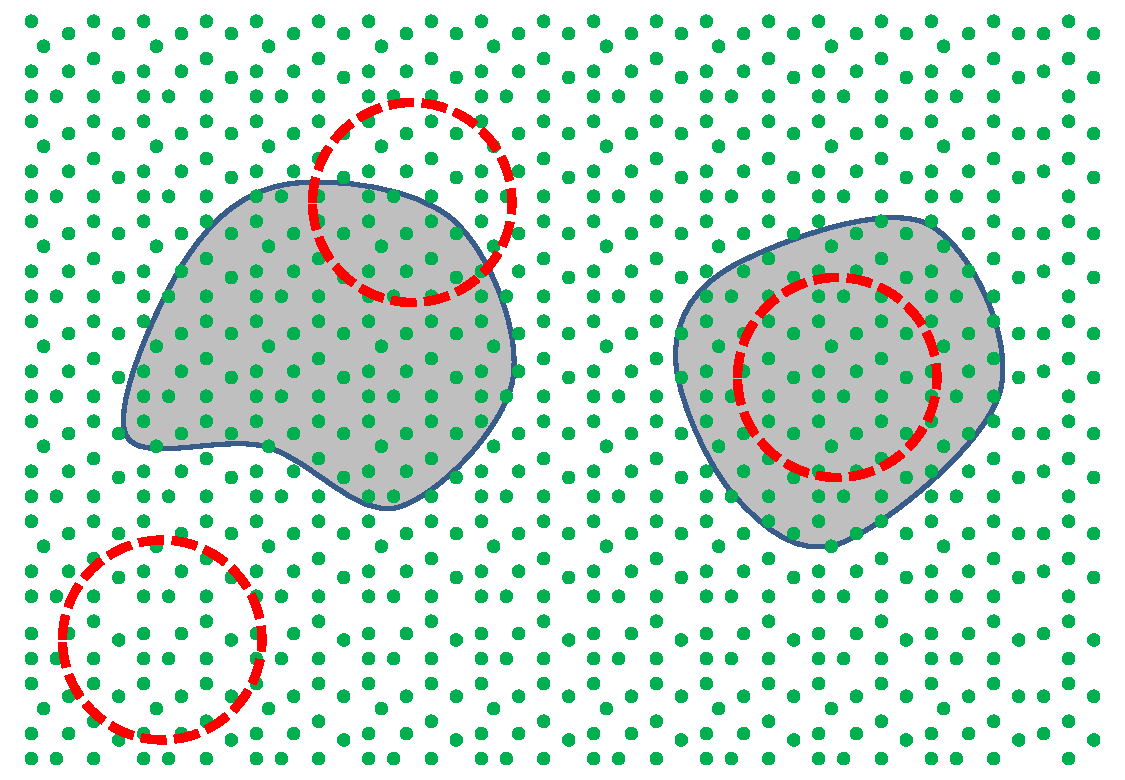
\includegraphics[width=\linewidth]{figs/5/collisionpacket.pdf}
\caption[Multiple configuration packet for parallel collision detection]{Multiple configuration packets for parallel collision detection. Green points are random configuration samples in $\mathcal{C}$-space. Grey areas are $\mathcal{C}$-obstacles. Configurations adjacent in $\mathcal{C}$-space are clustered into configuration packets (red circles). Some packets are completely in free space; some packets are completely within $\mathcal{C}$-obstacles; and some packets are near boundaries of $\mathcal{C}$-obstacles. Configurations in the
same packet have similar BVTT traversal paths and are mapped to the same warp on a GPU.}
  \label{fig:5:collisionpacket}
\end{figure}

Instead of solving Equation~(\ref{eq:5:cluster}) exactly, we use a simpler clustering scheme to compute an approximate solution. First, we use the $k$-means algorithm to cluster the $N$ queries into $C$ clusters, which can be implemented efficiently on GPUs~\cite{Che:2008}. Next, for $k = 1, ..., C$, we divide the $k$-th cluster of size $S_k$
into $\lceil \frac{S_k}{\text{chunk-size}}\rceil$ sub-clusters, each of which corresponds to a \emph{configuration-packet}. This simple method has some disadvantages. For example,
the number of clusters is $$\sum_{k=1}^C \lceil \frac{S_k}{\text{chunk-size}}\rceil \geq K = \lceil \frac{N}{\text{chunk-size}} \rceil$$, so we may not obtain an optimal solution for 
Equation~(\ref{eq:5:cluster}). However, as shown later, even this simple method can improve the performance
of parallel collision queries. The configuration clustering method is illustrated in
Figure~\ref{fig:5:collisionpacket}.

We then map each configuration-packet to a single chunk. Threads within one packet will traverse the BVTT synchronously; i.e., the algorithm works on one BVTT node $(x, y)$ at a time and processes the whole packet against the node. If $(x,y)$ is a leaf node, an exact intersection test is performed for each thread. Otherwise, the algorithm loads its children nodes and tests the BVs for overlap to determine the remaining traversal order, to select one child $(x_m, y_m)$ as the next BVTT node to be traversed for the entire packet. We select $(x_m, y_m)$ in a greedy manner: it corresponds to the child node that is classified as overlapping with the most threads in the packet. We also push other children into the packet's traversal stack. In the case that no BV overlap is detected in all the
threads or $(x,y)$ is a leaf node, $(x_m, y_m)$ would be the top element in the packet's traversal stack.  The traversal
step is repeated recursively, until the stack is empty. Compared to Algorithm~\ref{algo:5:naive}, all the threads in one chunk share one
traversal stack in shared memory, instead of using one stack for each thread. Therefore, the size of shared memory used
is reduced by the $\text{chunk-size}$ and results in higher parallel efficiency. The details of the traversal order decision rule are shown in Figure~\ref{fig:5:packettraverse}.

\begin{figure}[!htb]
  \centering
  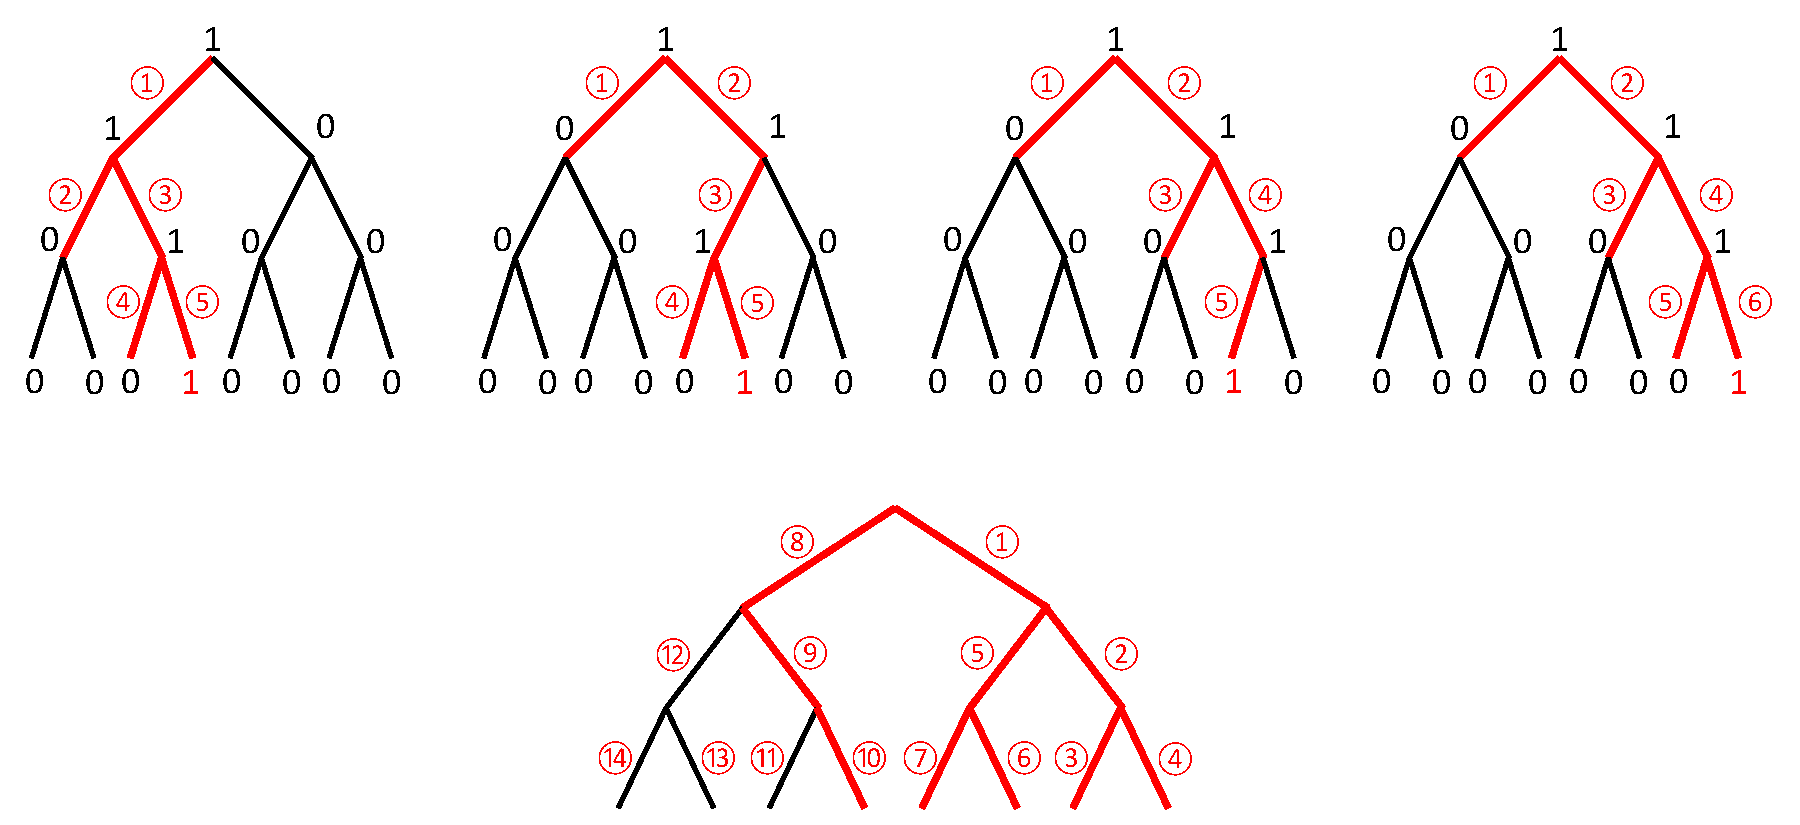
\includegraphics[width=\linewidth]{figs/5/packettraverse.pdf}
  \caption[Synchronous BVTT traversal for packet configurations]{Synchronous BVTT traversal for packet configurations. The four trees in the first row are the BVTT trees for configurations in the same chunk. For convenience, we represent BVTT as binary tree instead of 4-ary tree. The $1$ or $0$ at each node represents whether the BV-overlap or exact intersection test executed at that node is in-collision or collision-free. The red edges are the edges visited by the BVTT traversal algorithm and the indices on those edges
  represent the traversal order. In this case, the four different configurations have traversal paths of length $5$, $5$, $5$ and $6$. The leaf nodes with a red $1$ are locations where collisions are detected and the traversal stops.
  The tree in the second row shows the synchronous BVTT traversal order determined by our heuristic rule, which needs to visit $10$ edges to detect the collisions of all four configurations.}
  \label{fig:5:packettraverse}
\end{figure}

The traversal order described above is a greedy heuristic that tries to minimize the traversal path of the entire packet. For one BVTT node $(x,y)$, if no overlap is detected in any of the threads, it implies that these threads will not traverse the
sub-tree rooted at $(x,y)$. Since all the threads in the packet are similar and traverse the BVTT in nearly the same order,
this implies that other threads in the same packet may not traverse the sub-tree either. We define the probability that the sub-tree rooted at $(x,y)$ will be traversed by one thread as $$p_{x,y} = \frac{\text{number of overlap\ threads}}{\text{packet-size}}.$$ For any traversal pattern $P$ for BVTT, the probability that it is carried out by BVTT traversal will be $$p_P = \prod_{(x,y)\in P} p_{x,y}.$$
As a result, our new traversal strategy guarantees
that the traversal pattern with higher traversal probability will have a shorter traversal length, which therefore minimizes the overall
path for the packet.

The decision about which child node to choose for the next traversal step is computed using sum reduction~\cite{Mark:2009:sdk},
which can compute the sum of $n$ items in parallel with  $\mathcal{O}(\log(n))$ complexity. Each thread writes a $1$ in its own location in
the shared memory if it detects overlap in one child and $0$ otherwise. The sum of the memory locations is computed in
$5$ steps for  a size $32$ chunk, and the packet chooses the child node with the maximum sum. The complete algorithm for configuration-packet computation is described in Algorithm~\ref{algo:5:configuration-packet}.

\begin{algorithm}[htb]
    \caption{Multiple Configuration-Packet Traversal}
    \label{algo:5:configuration-packet}
    \begin{algorithmic}[1]
    \STATE Input: $N$ random configurations $\{\mathbf{q}_i\}_{i=1}^N$, BVH$_a$ for the robot and BVH$_b$ for the obstacles
    \STATE $t_{id} \leftarrow$ thread id of current thread
    \STATE $\mathbf{q} \leftarrow \mathbf{q}_{t_{id}}$
    \STATE \textbf{shared} $CN$[]$\equiv$ shared memory for children node
    \STATE \textbf{shared} $TS$[]$\equiv$ local traversal stack
    \STATE \textbf{shared} $SM$[]$\equiv$ memory for sum reduction
    \medskip
    \IF{$\overlap($BVH$_a(\mathbf{q})[1]$, BVH$_b[1])$ is \textbf{false} for all threads in chunk}
        \STATE \textbf{return}
    \ENDIF
    \STATE $(x,y) = (1,1)$
    \LOOP
        \IF{$\isLeaf(x)$ \&\& $\isLeaf(y)$}
        \IF{$\exactIntersect($BVH$_a(\mathbf{q})[x],$BVH$_b[y])$}
            \STATE update collision status of $\mathbf{q}$
        \ENDIF
        \IF{$TS$ is empty}
            \STATE \textbf{break}
        \ENDIF
        \STATE $(x,y) \leftarrow \pop(TS)$
        \ELSE \STATE $\lhd$ decide the next node to be traversed
            \STATE $CN$[] $\leftarrow (x,y)$'s children nodes
            \FORALL{$(x_c, y_c) \in CN$}
            \STATE $\lhd$ compute the number of threads that detect overlap at node $(x_c, y_c)$
            \STATE write $\overlap($BVH$_a(\mathbf{q})[x_c],$BVH$_b[y_c])$ (0 or 1) into $SM[t_{id}]$ accordingly
            \STATE compute local summation $s_c$ in parallel by all threads in chunk
            \ENDFOR
            \IF{$\max_c{s_c} > 0$}
            \STATE $\lhd$ select the node that is overlapped in the most threads
            \STATE $(x,y) \leftarrow CN[\argmax_c{s_c}]$ and push others into $TS$
            \ELSE
            \STATE $\lhd$ select the node from the top of stack
                \IF{$TS$ is empty}
                    \STATE \textbf{break}
                \ENDIF
                \STATE $(x,y) \leftarrow \pop(TS)$
            \ENDIF
        \ENDIF
    \ENDLOOP
    \end{algorithmic}
\end{algorithm}


\subsection{Parallel Collision Query with Workload Balancing}
Both Algorithms~\ref{algo:5:naive} and~\ref{algo:5:configuration-packet} use the per-thread per-query strategy, which is relatively easy to implement. However, when idle threads wait for busy threads or when the execution path of threads diverges, the parallel
efficiency on the GPUs decreases. Algorithm~\ref{algo:5:configuration-packet} can alleviate this problem in some cases, but it still distributes the tasks among the separate GPU cores and thus cannot make full use of the GPU's computational power.

In this section, we present the parallel collision query algorithm based on workload balancing, which further improves the performance. In this algorithm, the task of each thread is no longer one complete collision query or continuous collision query
(for local planning). Instead, each thread only performs BV overlap tests. In other words, the unit task for each thread is more fine-grained. 
Essentially, we formulate the problem of performing multiple collision queries as a pool of BV overlap tests which can be performed in parallel. It is easier to distribute these fine-grained tasks in a uniform manner onto all the GPU cores, thereby balancing the load among them, than to distribute the collision query tasks in a uniform manner.

All the fine-grained tasks are stored in large work queues in the GPU's main memory, which has a higher latency compared
to the shared memory. When computing a single collision query~\cite{Lauterbach10}, the tasks are in the form of
BVTT nodes $(x,y)$. Each thread will fetch several tasks from one work queue into its local work queue on the
shared memory and then will traverse the corresponding BVTT nodes. The children generated for each node are also pushed
into the local queue as new tasks. This process is repeated for all the tasks remaining in the queue,
until the number of threads with full or empty local work queues exceeds a given threshold (we use 50\%
in our implementation), at which point non-empty local queues are copied back to the work queues on main memory.
Since each thread performs simple tasks with few branches, our algorithm can make full use of GPU cores
if there are enough tasks in all the work queues. However, during the BVTT traversal, tasks
are generated dynamically and thus different queues may have varying numbers of tasks, which can lead to an uneven workload among the GPU cores. We use a balancing algorithm that redistributes the tasks among work queues (Figure~\ref{fig:5:balance}). Suppose the number of tasks in each work queue is $$n_i, 1\leq i \leq Q.$$ Whenever there exists $i$ so that $n_i < T_l$ or $n_i > T_u$, we execute our balancing algorithm among all the queues, which causes the number of tasks in each queue to be $$n_i^* = \frac{\sum_{k=1}^Q n_k}{Q}, 1\leq i \leq Q$$. $T_l$ and $T_u$ are two thresholds; we set $T_l$ to the $\text{chunk-size}$,
and set $T_u$ to $W-\text{chunk-size}$, where $W$ is the maximum size of the work queue.

We use several strategies in order to handle $N$ collision queries simultaneously, which are illustrated and compared in Figure~\ref{fig:5:gproximity-control}. One option is to repeat the single query algorithm~\cite{Lauterbach10} introduced above for each query. However, this has two main disadvantages. First, the GPU kernel has to be called $N$ times from the CPU, and this is expensive for large $N$ (which can be $\gg 10000$ for sample-based motion planning). Second, for each query, work queues are initialized with only one item (i.e., the root node of the BVTT); therefore, the GPU's computational power cannot be fully exploited at the beginning of each query, as shown in the slow ascending sections in Figure~\ref{fig:5:gproximity-control}(a). Similarly, at the end of each query, most tasks have been finished and some of the GPU cores become idle, which corresponds to the slow descending parts in Figure~\ref{fig:5:gproximity-control}(a).

As a result, we use the strategy shown in Figure~\ref{fig:5:gproximity-control}(b): we divide the $N$ queries into $\lceil\frac{N}{M}\rceil$ different sets each of size $M$ with $M\leq N$ and initialize the work queues with $M$ different BVTT roots for each iteration. Usually $M$ cannot be equal to $N$ because we need to use $t \cdot M$ Bytes GPU global memory to store the transform information for the queries, where the constant $t$ satisfies $$t \leq \frac{\text{size of global memory}}{M}$$ and we usually use $M=50$. In this case, we only need to invoke the solution kernel $\lceil\frac{N}{M}\rceil$ times. The number of tasks available in the work queues changes more smoothly over time, with shorter ascending and descending sections, which implies higher
throughput of GPUs. Moreover, the work queues are initialized with many more tasks, which results in high performance at the beginning of each iteration. In practice, as nodes from more than one BVTT of different queries co-exist in the same queue, we need to distinguish them by representing each BVTT node by $(x,y,i)$ instead of $(x,y)$, where $i$ is the index of collision query. The details for this strategy are shown in Algorithm~\ref{algo:5:balancing:task}.

We can further improve the efficiency by using the pump operation, as shown in Algorithm~\ref{algo:5:balancing} and Figure~\ref{fig:5:balance}. That is, instead of initializing a work queue after it is completely empty, we add $M$ BVTT root nodes of unresolved collision queries into a work queue when the number of tasks it contains drops below a threshold (we use $10\cdot \text{chunk-size}$). As a result, the few ascending and descending sections in Figure~\ref{fig:5:gproximity-control}(b) can be further flattened as shown in Figure~\ref{fig:5:gproximity-control}(c). The pump operation can reduce the timing overload of interrupting traversal kernels, as well as of copying data between global memory and shared memory, and therefore improves the overall efficiency of collision computation.


\begin{algorithm}[htb]
    \caption{Traversal with Workload Balancing: Task Kernel}
    \label{algo:5:balancing:task}
    \begin{algorithmic}[1]
    \STATE Input: abort signal $signal$, $N$ random configurations $\{\mathbf{q}_i\}_{i=1}^N$, BVH$_a$ for the robot and BVH$_b$ for the obstacles
    \STATE \textbf{shared} $WQ$[] $\equiv$ local work queue
    \STATE initialize $WQ$ by tasks in global work queues
    \STATE $\lhd$ traverse on work queues instead of BVTTs
    \LOOP
    \STATE $(x,y,i) \leftarrow \pop(WQ)$
    \IF{$\overlap($BVH$_a(\mathbf{q}_i)[x],$BVH$_b[y])$}
        \IF{$\isLeaf(x)$ \&\& $\isLeaf(y)$}
            \IF{$\exactIntersect($BVH$_a(\mathbf{q}_i)[x],$BVH$_b[y])$}
                \STATE update collision status of $i$-th query
            \ENDIF
        \ELSE
            \STATE $WQ$[] $\leftarrow (x,y,i)$'s children
        \ENDIF
    \ENDIF
    \IF{$WQ$ is full or empty}
    \STATE atomically increment $signal$, \textbf{break}
    \ENDIF
    \ENDLOOP
    \STATE \textbf{return} \textbf{if} $signal > 50\% Q $
    \end{algorithmic}
\end{algorithm}

\begin{algorithm}[htb]
    \caption{Traversal with Workload Balancing: Manage Kernel}
    \label{algo:5:balancing}
    \begin{algorithmic}[1]
    \STATE Input: $Q$ global work queues
    \STATE copy local queues on shared memory back to $Q$ global work queues on global memory
    \STATE compute the number of tasks in each work queue $n_i, 1\leq i\leq Q$
    \STATE compute the number of tasks in all queues $n = \sum_{k=1}^Q n_k$
    \IF{$n < T_{pump}$}
    \STATE call pump kernel: add more tasks in global queue from unresolved collision queries
    \ELSIF{$\exists i, n_i < T_l | | n_i > T_u$}
    \STATE call balance kernel: rearrange the tasks so that each queue has $n_i^* = \frac{\sum_{k=1}^Q n_k}{Q}$ tasks
    \ENDIF
    \STATE call task kernel again
    \end{algorithmic}
\end{algorithm}

\begin{figure}[!htb]
  \centering
  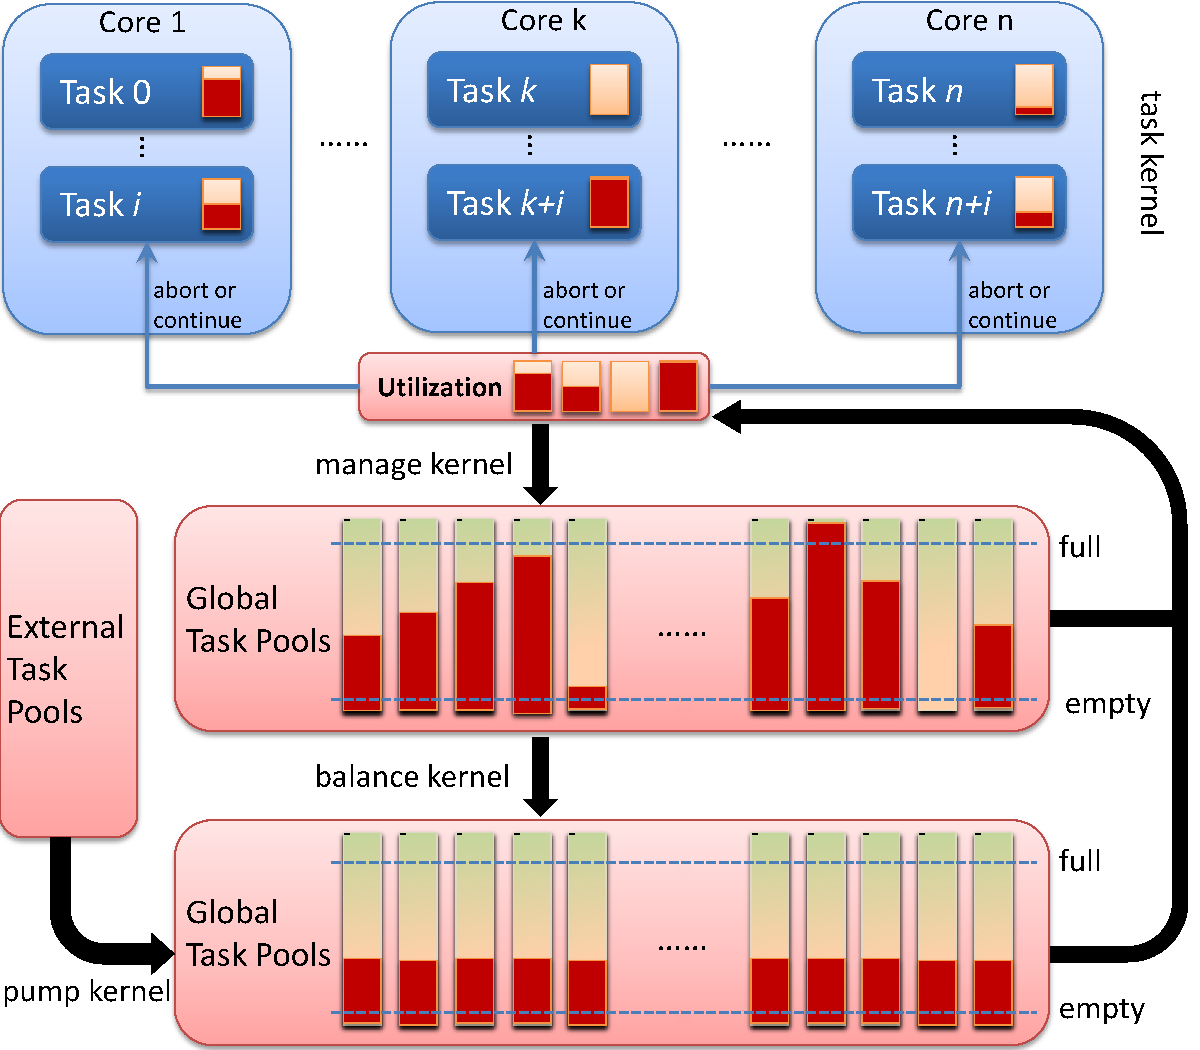
\includegraphics[width=\linewidth]{figs/5/balance.pdf}
  \caption[Load balancing strategy for our parallel collision query algorithm]{Load balancing strategy for our parallel collision query algorithm. Each thread keeps its own local work queue in local memory. After processing a task, each thread is either able to run further or has an empty or full work queue and terminates. Once the number of GPU cores terminated exceeds a given threshold, the \emph{manage kernel} is called and copies the local queues back onto global work queues. If no work queue has too many or too few tasks, the \emph{task kernel} restarts. Otherwise, the \emph{balance kernel} is called to balance the tasks among all the queues. If there are not sufficient tasks in the queues, more BVTT root nodes will be 'pumped' in by the \emph{pump kernel}.}
  \label{fig:5:balance}
\end{figure}

\begin{figure}[!htb]
  \centering
  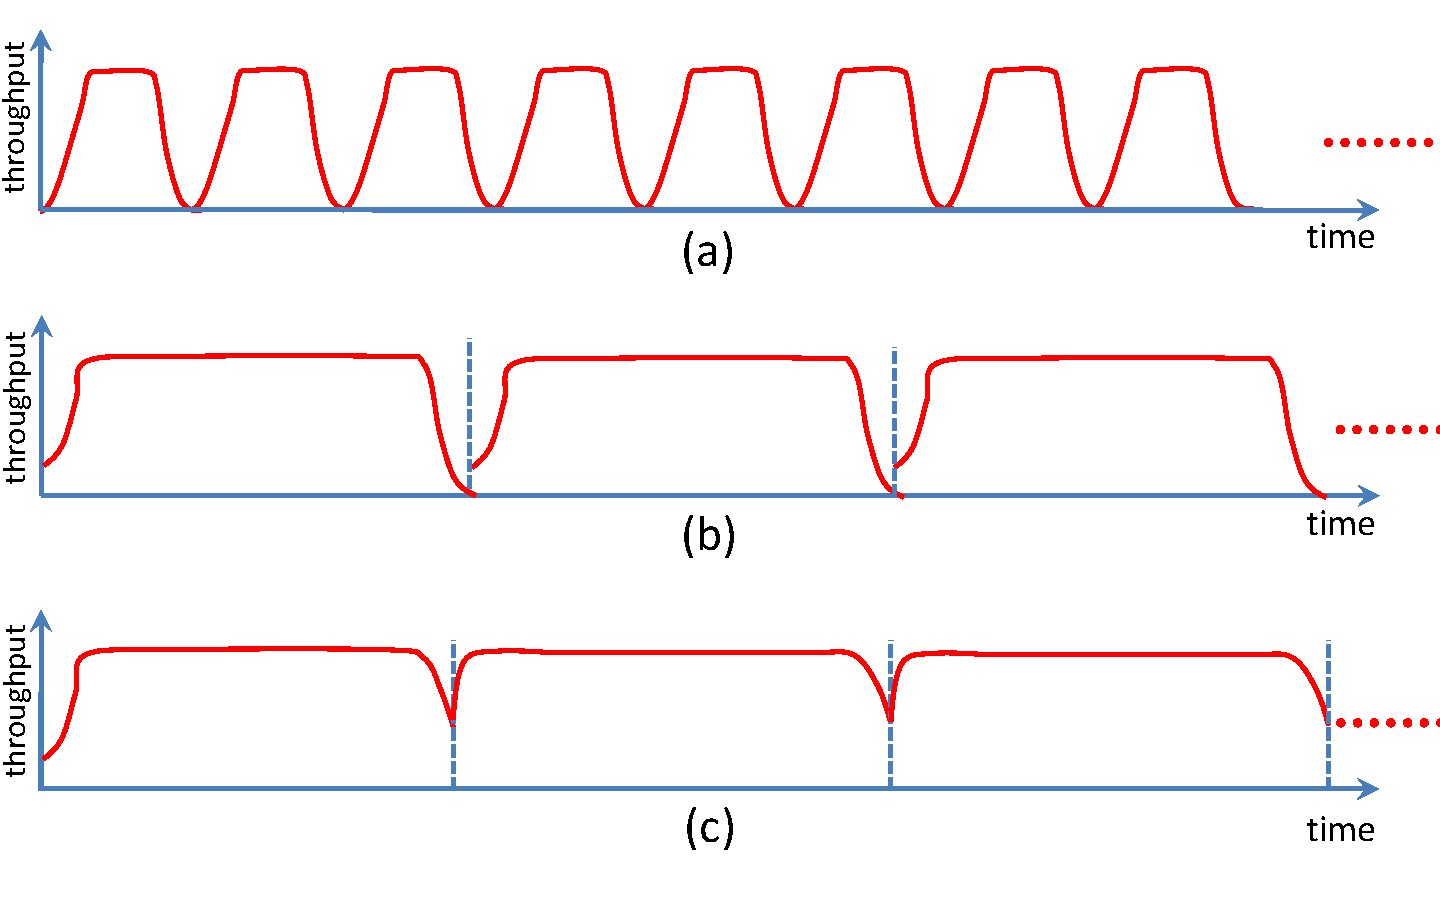
\includegraphics[width=\linewidth]{figs/5/gproximity-parallel-differentcontrol.pdf}
  \caption[Different strategies for parallel collision query using work queues]{Different strategies for parallel collision query using work queues. (a) Naive approach: repeat the single collision query algorithm. (b) Work queues are initialized with several BVTT root nodes and this process is repeated until all queries are performed. (c) is similar to (b) except that new BVTT root nodes are added to the work queues by the pump kernel, when there is not a sufficient number of tasks in the queue.}
  \label{fig:5:gproximity-control}
\end{figure}


\subsection{Analysis}

In this section, we analyze the algorithms described above using the \emph{parallel random access machine} (PRAM) model, which is a popular tool to analyze the complexity of parallel algorithms~\cite{Joesphbook}. Of course, current GPU architectures have many properties that can not be described by the PRAM model, such as SIMT, shared memory, etc. However, PRAM analysis can still provide some insight into a GPU algorithm's performance.

Suppose we are given $n$ collision queries, which means that we need to traverse $n$ BVTT of the same tree structure but with different geometry configurations. We denote the complexity of the serial algorithm as $T_S(n)$, the complexity of the naive parallel algorithm (Algorithm~\ref{algo:5:naive}) as $T_N(n)$, the complexity of the configuration-packet algorithm (Algorithm~\ref{algo:5:configuration-packet}) as $T_P(n)$ and the complexity of the workload balancing algorithm (Algorithm~\ref{algo:5:balancing}) as $T_B(n)$. Then we have the following result:

\begin{lemma}
\label{thm:5:analysis}
$\Theta(T_S(n)) = T_N(n) \geq T_P(n) \geq T_B(n)$.
\end{lemma}

\begin{remark} In parallel computing, we say one parallel algorithm is \emph{work efficient} if its complexity $T(n)$ is bounded both above and below asymptotically by $S(n)$, the complexity of its serial version, i.e., $T(n) = \Theta(S(n))$~\cite{Joesphbook}. In other words, Lemma~\ref{thm:5:analysis} means that all the three parallel collision algorithms are work-efficient, but the workload balancing is the most efficient and configuration-packet algorithm is more efficient than the naive parallel scheme.
\end{remark}

\begin{proof}
Let the complexity to traverse the $i$-th BVTT be $W(i)$, $1\leq i\leq n$. Then the complexity of a
sequential CPU algorithm is $T_S(n) = \sum_{i=1}^n W(i)$. For GPU-based parallel algorithms, we assume that the
GPU has $p$ processors or cores. For convenience, we assume $n = ap, a \in \mathbb{Z}$.

For the naive parallel algorithm (Algorithm~\ref{algo:5:naive}), each processor executes BVTT traversal independently and the overall performance is determined by the most time-consuming BVTT traversal. Therefore, its complexity becomes
$$T_N(n) = \sum_{k=0}^{a-1} \max_{j=1}^p W(kp + j).$$
If we sort $\{W(i)\}_{i=1}^n$ in ascending order and denote $W^*(i)$ as the $i$-th element in the new order, we have
\begin{equation}
\label{eq:5:lemma}
\sum_{k=0}^{a-1} \max_{j=1}^p W(kp + j) \geq \sum_{k=1}^{a}W^*(kp).
\end{equation}
To prove this, we start from $a=2$. In this case, the summation $\max_{j=1}^p W(j) + \max_{j=1}^p W(p + j)$ achieves the minimum when $\min{\{W(p+1), \cdots, W(2p)\}} \geq \max{\{W(1), \cdots, W(p)\}}$. Otherwise, exchanging the minimum value in $\{W(p+1), \cdots, W(2p)\}$ and the maximum value in $\{W(1), \cdots, W(p)\}$ will increase the summation. For $a>2$, using similar reasoning, we can show that the minimum of $\sum_{k=0}^{a-1} \max_{j=1}^p W(kp + j)$ happens when $\min_{k=jp+1}^{(j+1)p}{\{W(k)\}} \geq \max_{(j-1)p+1}^{jp}{\{W(k)\}}$, $1 \leq j \leq a - 1$. This is satisfied by the ascending sorted result $W^*$ and thus the inequality~(\ref{eq:5:lemma}) is proved.

Moreover, it is apparent that $\sum_{i=1}^n W(i) \geq T_N(n) \geq \frac{\sum_{i=1}^n W(i)}{p}$. Then we obtain
$$T_S(n) \geq T_N(n) \geq \max\big(\frac{T_S(n)}{p}, \sum_{k=1}^{a}W^*(kp)\big),$$
which implies $T_N(n) = \Theta(T_S(n))$.

According to the analysis in Section~\ref{sec:5:algorithm:packet}, we know that the expected complexity $\hat{W}(i)$ for $i$-th BVTT traversal in configuration-packet method (Algorithm~\ref{algo:5:configuration-packet}) should be smaller than $W(i)$ because of the near-optimal traversing order. Moreover, the clustering strategy is similar to ordering different BVTTs, so that the BVTTs with similar traversal paths are arranged closely to each other and thus the probability is higher that they would be distributed on the same GPU core. In practice, we can not implement such an ordering exactly
because the complexity of BVTT traversal is not known a priori. Therefore the complexity of Algorithm~\ref{algo:5:configuration-packet} is $$T_P(n) \approx \sum_{k=1}^a \hat{W}^*(kp),$$ with $\hat{W}^* \leq W^*$. As a result, we have $T_P(n) \leq T_N(n)$.

The complexity for the workload balancing method (Algorithm~\ref{algo:5:balancing}) can be given as: $$T_B(n) = \frac{\sum_{i=1}^n W(i)}{p} + B(n),$$ where the first item is the time complexity for BVTT traversal and the second item $B(n)$ is the time complexity for the balancing step. As $B(n) > 0$, the acceleration ratio of GPU with $p$-processors is less than $p$. We need to reduce the load of the balancing step to improve the efficiency of Algorithm~\ref{algo:5:balancing}. If balancing step is implemented efficiently: i.e., if $B(n) = \mathcal O (T_S(n))$, we have $T_N(n) \geq T_P(n) \geq T_B(n)$.
\end{proof}



\section{Implementation and Results}
\label{sec:5:result}


In this section, we present details of the implementation and evaluate the performance of our algorithm
on different benchmarks. All the timings reported here were recorded on a machine using an Intel Core i7 3.2GHz CPU and 6GB
memory. We implemented our collision and planning algorithms using CUDA on a NVIDIA GTX 480 GPU with 1GB of video memory.

\subsection{GPU-based Planner}
We use the motion planning framework called \emph{gPlanner} introduced in Chapter~\ref{chp:GPlanner}, which uses PRM
as the underlying planning algorithm since it is more suitable to exploit the multiple cores and data parallelism on GPUs. gPlanner is completely implemented on GPUs to avoid the expensive data transfer the between CPU and GPU.


\subsection{Implementation}
As part of our implementation, we replace the collision detection module in gPlanner with the new algorithms described above.
As observed in Chapter~\ref{chp:GPlanner}, motion planning algorithms spend more than 
90\% of their time in collision queries, i.e., milestone computation and local planning.

\begin{table}[!htb]
\begin{center}
\begin{tabular}{|c|c|c|c|c|c|}\hline
&piano & large-piano & helicopter & humanoid & PR2 \\ \hline \hline
\#faces of the robot mesh & 6,540 & 34,880 & 3,612 &  27,749 & 31,384\\ \hline
\#faces of the obstacle mesh & 648 & 13,824 & 2,840 & 3,495 & 3,495\\ \hline
DOF & 6 & 6 & 6 & 38 & 12 (one arm) \\ \hline
\end{tabular}
\caption[Geometric complexity of benchmarks for testing GPU-based collisions]{Geometric complexity of our benchmarks. Large-piano is a piano model that has more vertices and faces and is obtained by subdividing the original piano model.}
\label{tab:5:geom-complexity}
\end{center}
\end{table}

\begin{figure}[!htb]
    \subfloat[piano]{\centering 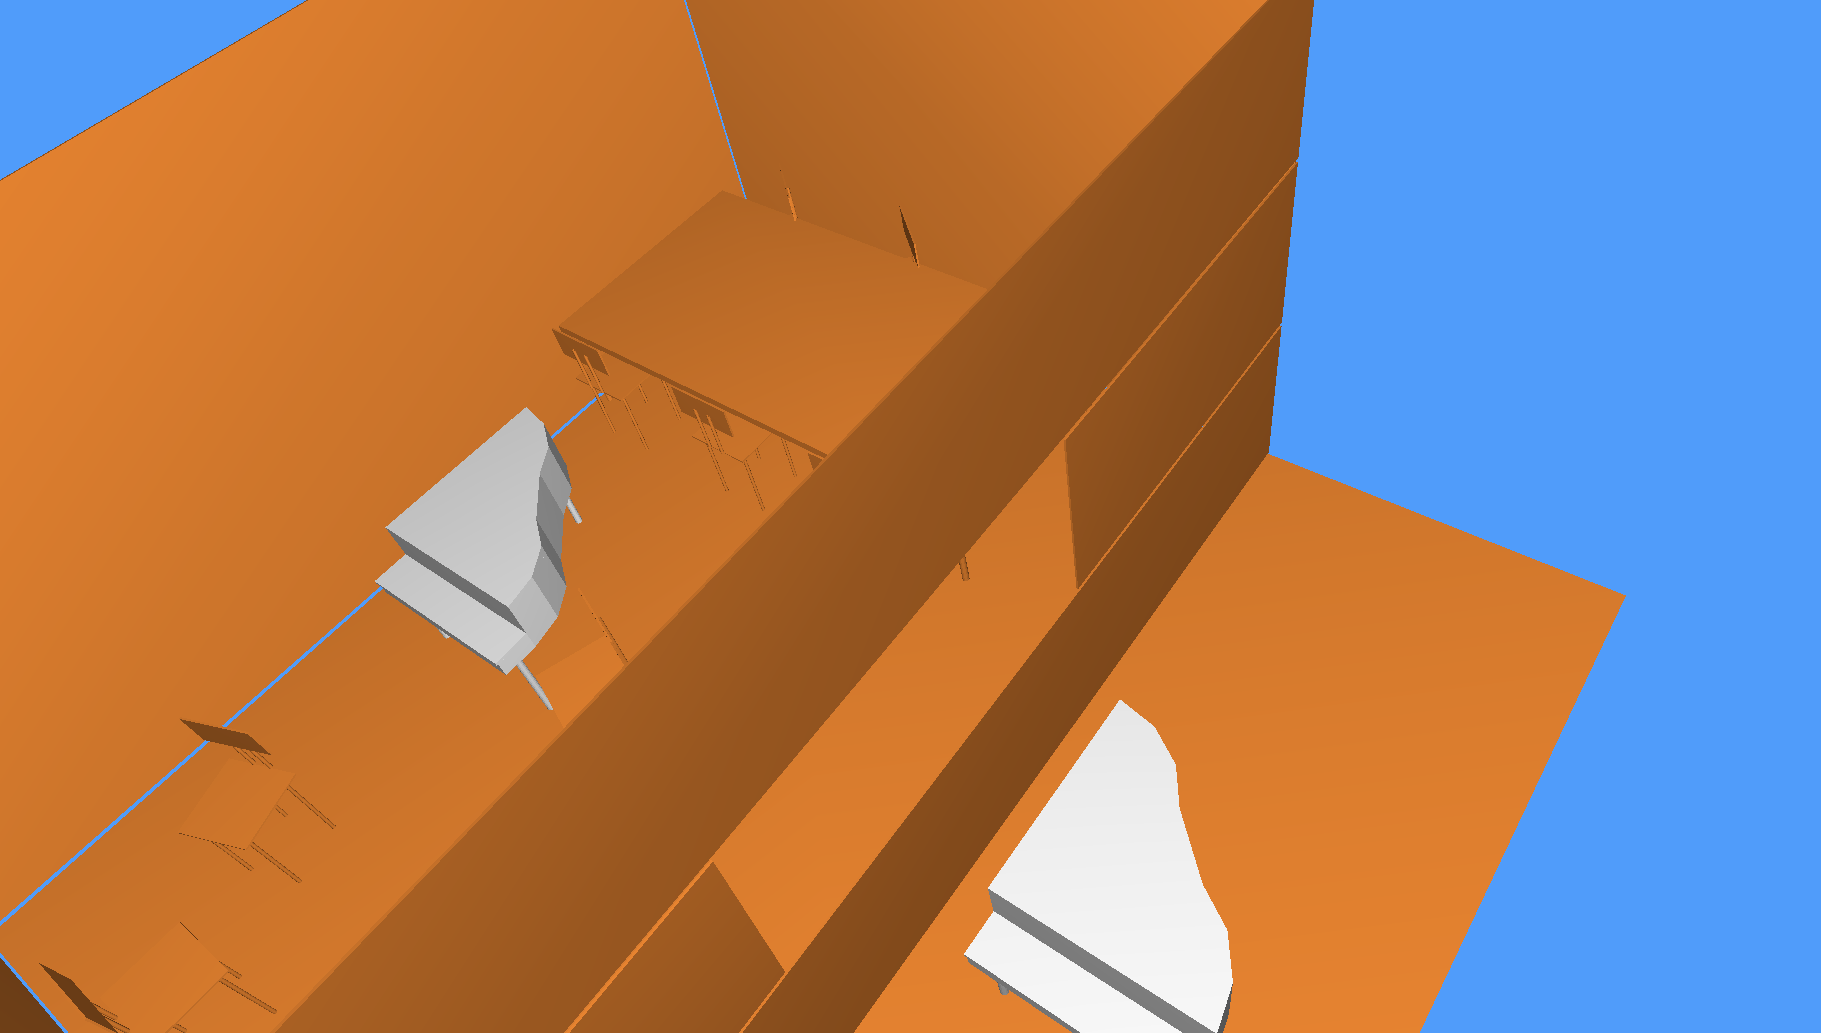
\includegraphics[width=0.3\linewidth]{figs/5/piano.png}}
    \subfloat[helicopter]{\centering 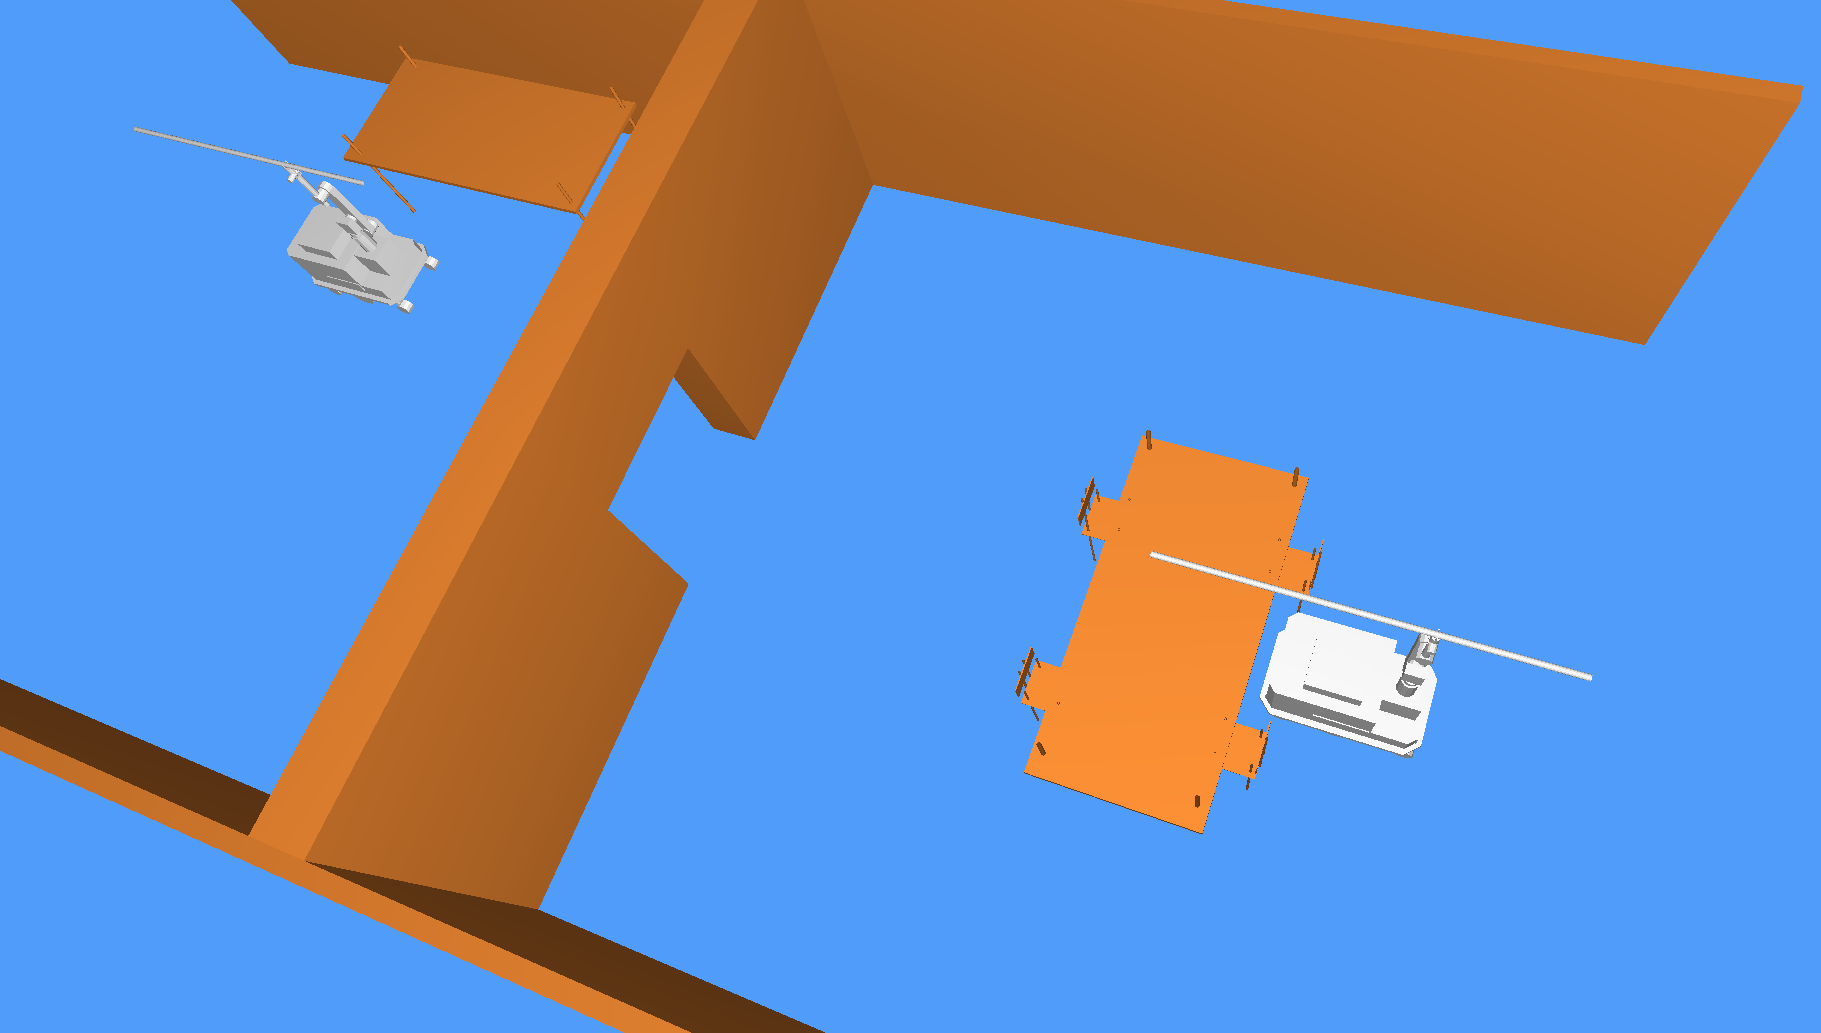
\includegraphics[width=0.3\linewidth]{figs/5/helicopter.png}}
    \subfloat[humanoid]{\centering 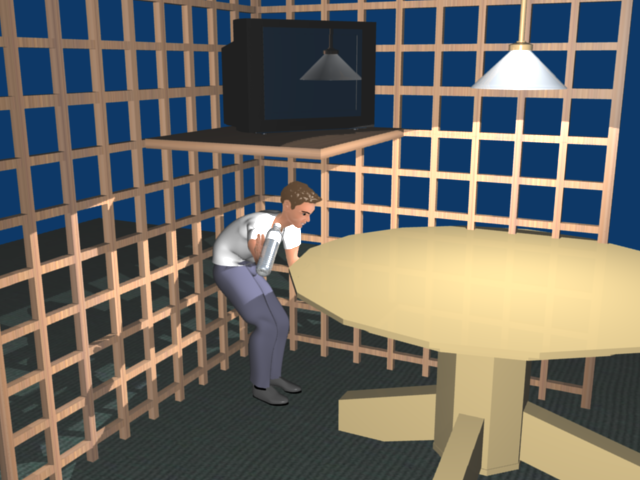
\includegraphics[width=0.23\linewidth]{figs/5/pick.png}}
    \subfloat[PR2]{\centering 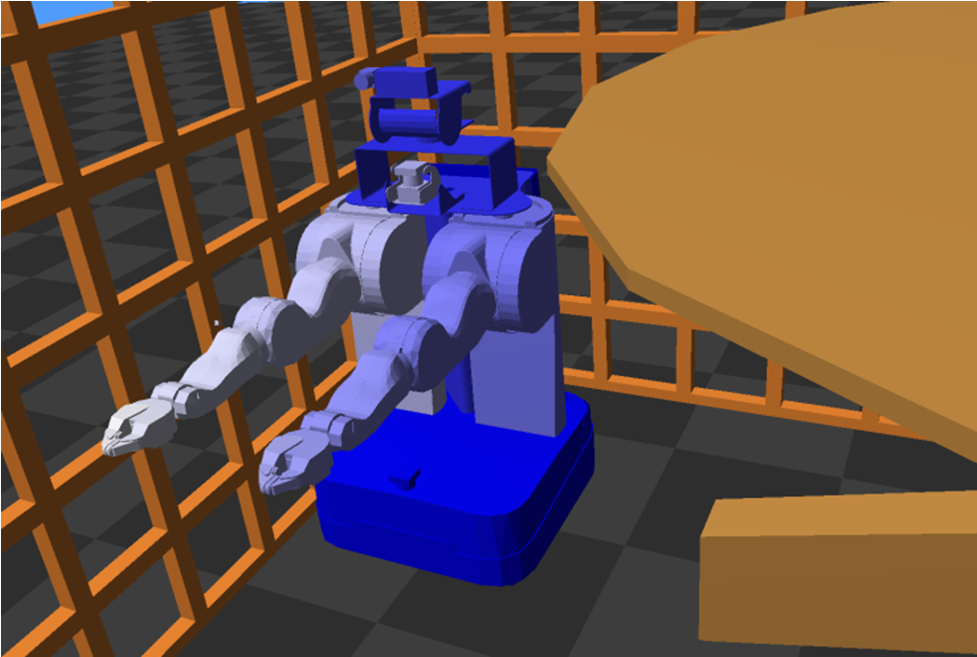
\includegraphics[width=0.26\linewidth]{figs/5/pr2.png}}
    \caption[Benchmarks used for testing GPU-based parallel collisions]{Benchmarks used in our experiments.}
    \label{fig:5:benchmarks}
\end{figure}

In order to compare the performance of different parallel collision detection algorithms, we use the benchmarks shown
in Figure~\ref{fig:5:benchmarks}. The geometric complexity of these benchmarks is shown in  Table~\ref{tab:5:geom-complexity}.
For rigid body benchmarks, we generate $50,000$ random configurations and compute a collision-free path by using different
variants of our parallel collision detection algorithm. For articulated model benchmarks, we generate $100,000$
random configurations. For milestone computation, we directly use our collision
detection algorithm. For local planning, we first need to unfold all the interpolated configurations: we denote the
BVTT for the $j$-th interpolated query within the $i$-th local path as BVTT$(i,j)$ and its node as $(x,y,i,j)$.
In order to avoid unnecessary computations, we first add BVTT root nodes with small $j$ into the work queues; $(1,1,i,j) \prec (1,1,i',j')$, if$j < j'$. As a result, once a collision is computed at BVTT$(i, j_0)$,
we need not traverse BVTT$(i, j)$ when $j > j_0$.

For Algorithms~\ref{algo:5:naive} and~\ref{algo:5:configuration-packet}, we further test the performance for
different traversal stack sizes ($32$ and $128$). Both algorithms give correct results when using a larger stack size ($128$). For smaller stack sizes, the algorithms will stop once the stack is filled.
Algorithm~\ref{algo:5:naive} may report a collision when the stack overflows, while Algorithm~\ref{algo:5:configuration-packet}
returns a collision-free query. Thus, Algorithm~\ref{algo:5:naive} may suffer from false positive errors while Algorithm~\ref{algo:5:configuration-packet}
may suffer from false negative errors. We also
compare the performances of Algorithm~\ref{algo:5:naive} and Algorithm~\ref{algo:5:configuration-packet} when the clustering algorithm described in Section~\ref{sec:5:algorithm:packet} is used and when it is not.

\begin{figure}[!htb]
  \centering
  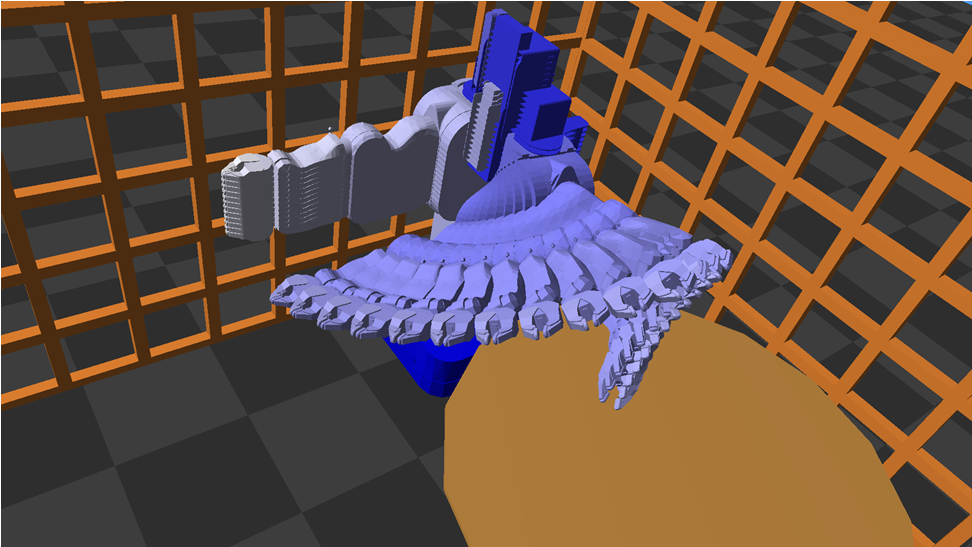
\includegraphics[width=\linewidth]{figs/5/pr2_result.png}
  \caption[The GPU-based motion planner can compute a collision-free path for PR2 in less than $1$ second]{Our GPU-based motion planner can compute a collision-free path for PR2 in less than $1$ second. }
  \label{fig:5:PR2result}
\end{figure}


\begin{table}[!htb]
\begin{center}
\resizebox{\linewidth}{!}{%
\begin{tabular}{|c|c|c|c|c|c|c|c|c|c|c|} \hline
     \multicolumn{1}{|c}{} & \multicolumn{4}{|c}{Algorithm~\ref{algo:5:naive}} & \multicolumn{4}{|c}{Algorithm~\ref{algo:5:configuration-packet}} & \multicolumn{2}{|c|}{Algorithm~\ref{algo:5:balancing}}\\ \hline \hline
\multicolumn{1}{|c|}{} & 32, no-C & 32, C & 128, no-C & 128, C & 32, no-C & 32, C & 128, no-C & 128, C & traversal & balancing \\ \hline \hline
piano & 117 & 113 & 239 & 224 & 177 & 131 & 168 & 130 & 68 & 3.69 \\ \hline
large-piano & 409 & 387 & 738 & 710 & 613 & 535 & 617 & 529 & 155 & 15.1 \\ \hline
helicopter & 158 & 151 & 286 & 272 & 224 & 166 & 226 & 163 & 56 & 2.3 \\ \hline
humanoid & 2,392 & 2,322 & 2,379 & 2,316 & 2,068 & 1,877 & 2,073 & 1,823 & 337 & 106 \\ \hline
\end{tabular}
}
\end{center}
\caption[Comparison of different CPU-based and GPU-based algorithms in the milestone computation component of PRM motion planner]{Comparison of different algorithms in milestone computation (timing in milliseconds). 32 and 128 are the
different sizes used for the traversal stack; C and no-C refer to using pre-clustering and not using pre-clustering, respectively; the timing of Algorithm~\ref{algo:5:balancing} includes two parts: traversal and balancing.}\label{tab:5:milestone}
\end{table}

\begin{table}[!htb]
\begin{center}
\resizebox{\linewidth}{!}{%
\begin{tabular}{|c|c|c|c|c|c|c|c|c|c|c|} \hline
     \multicolumn{1}{|c}{} & \multicolumn{4}{|c}{Algorithm~\ref{algo:5:naive}} & \multicolumn{4}{|c}{Algorithm~\ref{algo:5:configuration-packet}} & \multicolumn{2}{|c|}{Algorithm~\ref{algo:5:balancing}}\\ \hline \hline
\multicolumn{1}{|c|}{} & 32, no-C & 32, C & 128, no-C & 128, C & 32, no-C & 32, C & 128, no-C & 128, C & traversal & balancing \\ \hline \hline
piano & 1,203 & 1,148 & 2,213 & 2,076 & 1,018 & 822 & 1,520 & 1,344 & 1,054 & 34 \\ \hline
large-piano & 4,126 & 3,823 & 8,288 & 7,587 & 5,162 & 4,017 & 7,513 & 6,091 & 1,139 & 66 \\ \hline
helicopter & 4,528 & 4,388 & 7,646 & 7,413 & 3,941 & 3,339 & 5,219 & 4,645 & 913 & 41 \\ \hline
humanoid & 5,726 & 5,319 & 9,273 & 8,650 & 4,839 & 4,788 & 9,012 & 8,837 & 6,082 & 1,964 \\ \hline
\end{tabular}
}
\end{center}
\caption[Comparison of different CPU-based and GPU-based algorithms in the local planning component of PRM motion planner]{Comparison of different algorithms in local planning (timing in milliseconds). 32 and 128 are the
different sizes used for the traversal stack; C and no-C means refer to pre-clustering and not using pre-clustering, respectively; the timing of Algorithm~\ref{algo:5:balancing} includes two parts: traversal and balancing.}\label{tab:5:localplanning}
\end{table}

The timing results are shown in Table~\ref{tab:5:milestone} and Table~\ref{tab:5:localplanning}. We make two main observations. First, Algorithms~\ref{algo:5:naive} and~\ref{algo:5:configuration-packet} both work better when the local traversal stack is smaller and the pre-clustering technique is used. However, for large models, a traversal stack of size $32$ may lead to overflows, and the
collision results may be incorrect, which happens for the large-piano benchmark in Table~\ref{tab:5:milestone} and Table~\ref{tab:5:localplanning}. Algorithm~\ref{algo:5:naive}'s performance is considerably reduced when the size of traversal stack
increases to $128$. This is due to the fact that Algorithm~\ref{algo:5:configuration-packet} uses per-packet stack,
which is about $32$ times smaller then using per-thread stack. Moreover, clustering and  configuration-packet traversal
can result in more than 50\% speed-up. The improvement in the performance of
Algorithm~\ref{algo:5:configuration-packet} over Algorithm~\ref{algo:5:naive} is more noticeable on complex models (e.g., large-piano).
Second, we observe that Algorithm~\ref{algo:5:balancing} is usually the fastest among all variations of the three algorithms.
It can result in more than 5-10 times speedup over other methods.


\begin{figure}[!h]
  \centering
  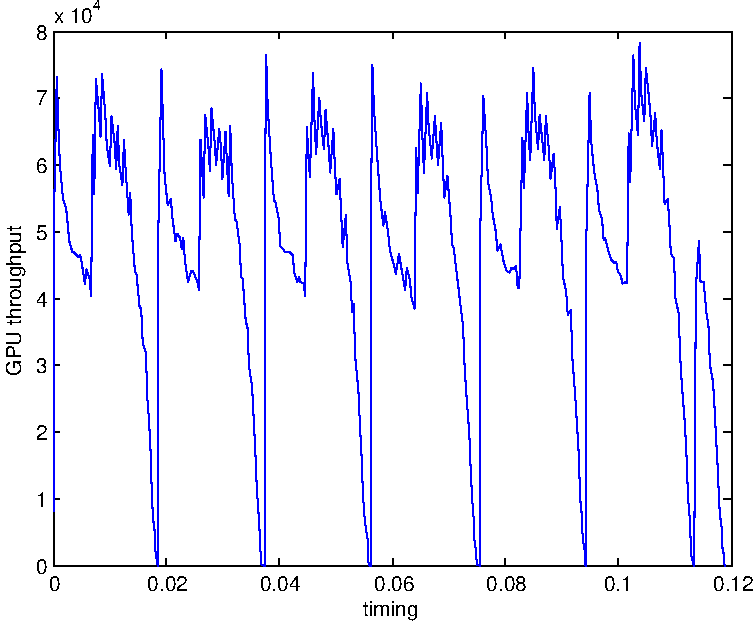
\includegraphics[width=0.8\linewidth]{figs/5/nopump.pdf}
  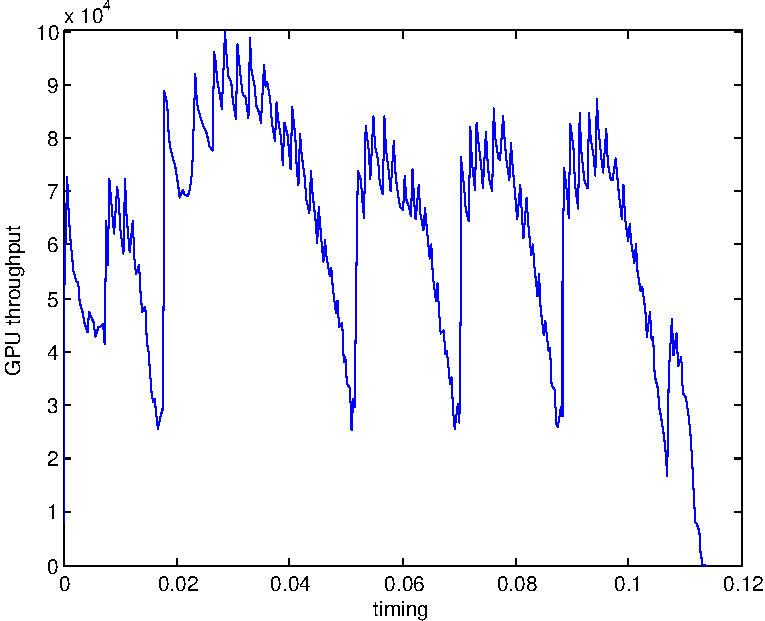
\includegraphics[width=0.8\linewidth]{figs/5/pump.pdf}
  \caption[GPU throughput improvement caused by pump kernel]{GPU throughput improvement caused by the pump kernel. The left figure shows throughput without using the pump kernel
  and the right figure shows throughput using the pump kernel.}
  \label{fig:5:pump}
\end{figure}

As observed in Chapter~\ref{chp:GPlanner}, the performance of the planner in these benchmarks is
dominated by milestone computation and local planning. Based on the novel collision detection algorithm, the performance of PRM
and lazy PRM planners can be improved by at least 40-45\%.

In Figure~\ref{fig:5:pump}, we also show how the pump kernel increases the GPU throughput (i.e., the number of
tasks available in work queues for GPU cores to fetch) in the workload-balancing-based Algorithm~\ref{algo:5:balancing}.
The maximum throughput (i.e., the maximum number of BV overlap tests performed by GPU kernels) increases from $8\times 10^4$
to nearly $10^5$, and the minimum throughput increases from $0$ to $2.5\times 10^4$. For the piano and helicopter models,
we can compute a collision-free path from the initial to the goal configuration in $879$ms and $778$ms, respectively,
using PRM and $72.79$ms or $72.68$ms, respectively, using lazy PRM.


\subsection{Articulated Models}
Our parallel algorithms can be directly applied to articulated models. In this case, checking for self-collisions among
various links of a robot adds to the overall complexity. We use a model of the PR2 robot as an articulated
benchmark. The PR2 robot model has 65 links and 75 DOFs. We only allow one arm (i.e., 12 DOFs) to be active in terms
of motion. A naive approach would involve exhaustive self-collision checking, and reduces to checking
$65 \times (65-1)/2 = 2,080$ self-collisions among the links for each collision query.
As shown in Table~\ref{tab:5:selfcollision}, GPU-based planner takes more than $10$ seconds for the PR2 benchmark when
performing exhaustive self-collision checking, though it is still much faster than the CPU-based implementation.

However, exhaustive self-collision checking is usually not necessary for  physical robots, because the joint limits can
filter out many of the self-collisions. The common method is to manually set link pairs that need to be checked
for self-collisions. This strategy can greatly reduce the number of pairwise checks. As shown in Table~\ref{tab:5:selfcollision}, we can compute a collision-free path for the PR2 model in less than $1$ second, which can be further reduced to $300$ms if
the number of samples is reduced to $500$. The collision-free path calculated by our planner is shown in Figure~\ref{fig:5:PR2result}.


\begin{table}[!htb]
\begin{center}
\begin{tabular}{|c|c|c|} \hline
                                & milestone computation & local planning \\ \hline
exhaustive self-collision (CPU) & 15,952 & 643,194 \\ \hline
exhaustive self-collision (GPU) & 652 & 13,513 \\ \hline
manual self-collision (GPU) & 391 & 392 \\ \hline
\end{tabular}
\end{center}
\caption[Comparison of the collision timing on PR2 benchmark when using CPU-based and GPU-based collision checking algorithms]{Collision timing on PR2 benchmark (timing in milliseconds). We use $1,000$ samples, $20$-nearest neighbor, and discrete local planning with $20$ interpolations. Manually specifying self-collisions can greatly improve the performance of the GPU planner. }\label{tab:5:selfcollision}
\end{table}


\section{Conclusion and Future Work}
In this chapter, we introduce two novel parallel collision query algorithms for real-time motion planning on GPUs.
The first algorithm is based on configuration-packet tracing, is easy to implement, and can improve parallel
performance by performing more coherent traversals and reducing the memory consumed by traversal stacks. It can provide
more than 50\% speed-up compared to simple parallel methods. This second algorithm is based on workload balancing, and
decomposes parallel collision queries into fine-grained tasks corresponding to  BVTT node operations. The algorithm
uses a light-weight task-balancing strategy to guarantee that all GPU cores are fully utilized and achieves
close to peak performance on GPUs. In practice, we observe 5-10 times speed-up. These new collision algorithms can improve
the performance of GPU-based PRM planners by almost 50\%.

There are many avenues for future work. We are interested in using more advanced sampling schemes with the
GPU-based planner to further improve its performance and deal with narrow passages. Furthermore, we would like to
modify the planner to generate smooth paths and integrate our planner with physical robots (e.g., PR2).
We would also like to take into account kinematic and dynamic constraints.
